% !TEX root = ./main.tex

\documentclass{article}
\usepackage[utf8]{inputenc}
\usepackage{pdfpages}
\usepackage{graphicx}
\graphicspath{ {./img/} }

\usepackage{listings}
\usepackage{xcolor}

\definecolor{codegreen}{rgb}{0,0.6,0}
\definecolor{codegray}{rgb}{0.5,0.5,0.5}
\definecolor{codepurple}{rgb}{0.58,0,0.82}
\definecolor{backcolour}{rgb}{0.95,0.95,0.92}

\lstdefinestyle{mystyle}{
    backgroundcolor=\color{backcolour},   
    commentstyle=\color{codegreen},
    keywordstyle=\color{magenta},
    numberstyle=\tiny\color{codegray},
    stringstyle=\color{codepurple},
    basicstyle=\ttfamily\footnotesize,
    breakatwhitespace=false,         
    breaklines=true,                 
    captionpos=b,                    
    keepspaces=true,                 
    numbers=left,                    
    numbersep=5pt,                  
    showspaces=false,                
    showstringspaces=false,
    showtabs=false,                  
    tabsize=2
}

\lstset{style=mystyle}
\lstset{literate=%
{Ö}{{\"O}}1
{Ä}{{\"A}}1
{Ü}{{\"U}}1
{ß}{{\ss}}2
{ü}{{\"u}}1
{ä}{{\"a}}1
{ö}{{\"o}}1
}


\title{Aktorik Sensorik \\ Labor 1}
\author{Anton Kress (S872899), Jan Abel (S876662)}
\date{October 2020}

\begin{document}

\maketitle


\section*{Aufgabenstellung}

\begin{figure}[htp]
 \centering
 \includegraphics[page=3, width=0.8\textwidth]{Aufgabenstellung.pdf}
 %\caption{Aufbau der CBM-Toolchain}
 \label{fig:Aufgabenstellung A1}
\end{figure}


\section{Messung des Stillstandsdrehmomentes}

\begin{figure}[htp]
 \centering
 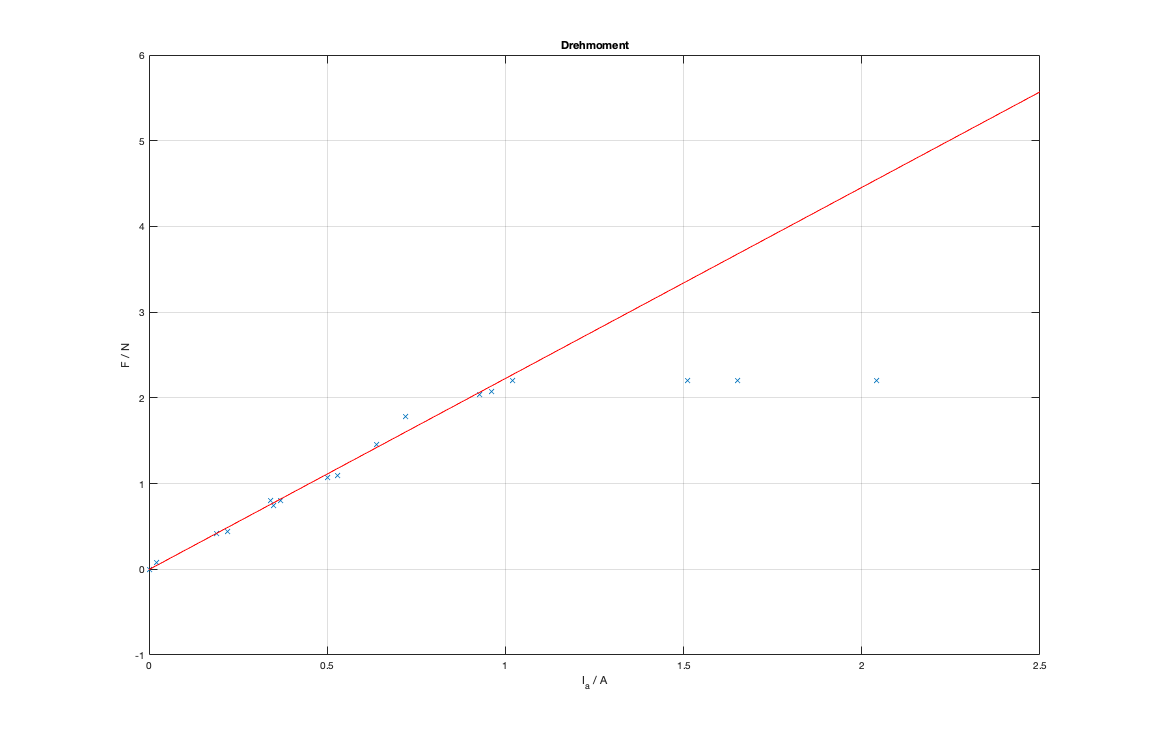
\includegraphics[width=1\textwidth]{a_1-1.png}
 \caption{Aufbau der CBM-Toolchain}
 \label{fig:Schnittstellen_IGX-560}
\end{figure}

\lstinputlisting[language=Matlab]{./src/A1.m}


blablabla
\section{Messung des Ankerwiderstandes}
\section{Messung der Leerlaufkennlinie}
\section{Messung der Kennlinie des Leistungsverstärkers}

\end{document}
